\documentclass[border=0.5mm]{standalone}

\usepackage{import}
\subimport{../../../}{preamble.tex}

\usepackage{tikz}
\usetikzlibrary{calc}

\usepackage{pgfplots}
\usepgfplotslibrary{fillbetween}

\begin{document}

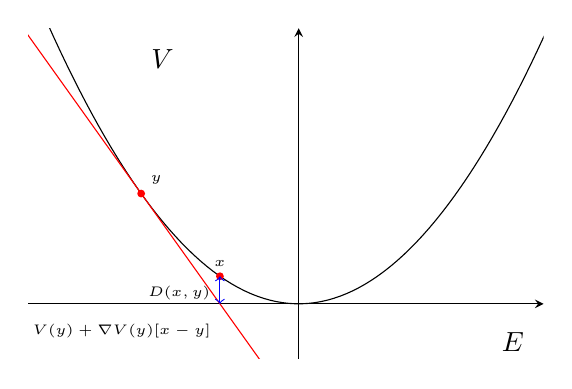
\begin{tikzpicture}

  \begin{axis}[
    ticks=none,
    axis lines=center,
    y=0.7cm,            % y unit vector
    x=1cm,            % x unit vector
    clip=true,
    ymax=5,
    ymin=-1,
    xlabel={ $E$},
    ylabel={ $V$},
    x label style={at={(axis description cs:0.9,0.05)},anchor=west},
    y label style={at={(axis description cs:0.22,0.85)},anchor=south west},
    ]
    
    \addplot[mark=none, black, samples=100, domain=-4:4] { x*x/2 };

    \addplot[mark=none, red, samples=100, domain=-4:4] { 2-2*(x+2) };
    \node[right] at (axis cs:-3.5, -0.5) {\tiny \red{$V(y) + \nabla V(y)[x-y]$}};

    \node[circle, inner sep=1, fill=red] (x) at (axis cs:-2, 2) {};
    \node[above right] at (x) {\tiny \red{$y$}};

    \node[circle, inner sep=1, fill=red] (y) at (axis cs:-1, 1/2) {};
    \node[above] at (y) {\tiny \red{$x$}};

    \node (y_a) at (axis cs:-1, 0) {};

    \node[left] at (axis cs:-1, 0.2) {\tiny \blue{$D(x, y)$}};

    \draw[<->, blue] (y_a.center) -- (y.center) ;
    
  \end{axis}
  
\end{tikzpicture}

\end{document}

%%% Local Variables:
%%% mode: latex
%%% TeX-master: t
%%% End:
